\selectlanguage{english}
\begin{abstract}
    \noindent A \emph{Számítógépes szimulációk} laboratórium harmadik alkalmával az egyszerű bolygómozgással és a Kepler-problémával kapcsolatos numerikus módszereket vizsgáltuk. Összehasonlítottuk, hogy az eddigi szimulációkban is már használt adaptív lépéshosszváltó módszer milyen körülmények mellett alkalmas az említett problémák differenciálegyenleteinek megoldására és hogy viselkedik különböző kezdőparaméterek hatására. Emellett megvizsgáltuk futásidejét is a fix lépéshosszal integráló módszerrel kontrasztba állítva. \\
    Modelleztük az egy-, a két- és háromtest-problémát, valamint megvizsgáltuk a Merkúr perihélium-precesszióját, kiegészítve a mozgásegyenleteket relativisztikus effektusokkal is. Végül a háromtest-probléma esetén modelleztük a Nap-Jupiter rendszerben található aszteroidák és meteorrajok mozgását és a Lagrange-pontokban kialakuló egyensúlyát.
\end{abstract}
\selectlanguage{magyar}

\begin{multicols}{2}

\section{Feladatok} \label{sec:1}
A kurzus harmadik alkalmával a bolygómozgás témáját jártuk részletesen körül, vizsgálva annak mind a kepleri, mind pedig az einsteini, relativisztikus hatásokkal kibővített modelljét is.\\
Előzetesen az egytest probléma kepleri mozgásegyenletét megoldani képes keretrendszer volt számunkra megadva. Ezt felhasználva kellett első lépésben ellenőrizzük, hogy a szimuláció mennyire stabil a numerikus hibákra, tehát az integrálási módszer, a lépésköz és az adaptív pontosság megválasztására. Én ezt vizsgálandó, a Nap-Merkúr rendszer keringését vizsgáltam, azon belül is pontosan a Merkúr ellipszispályájának potenciális elfordulását. Triviálisan azt várnánk, hogy a gravitációs kölcsönhatás klasszikus leírását alkalmazva, egy periódus megtétele után ugyanabba a pontba érkezik vissza egy bolygó keringése során. Ezzel szemben a relativisztikus tárgyalás esetén az égitestek mozgása erős gravitációs térben másabb, így pl. a Merkúr nagytengelye időben elfordul nem záródik. A Merkúr esetében ez a modern adatok ismeretében $100$ év ($\approx 415$ periódus) alatt $\approx 43"$-es precessziót jelent (Magnan, 2007\cite{2007arXiv0712.3709M}; Biesel, 2008\cite{biesel2008precession}) az eredeti állapothoz képest. Ennek alakulását vizsgálva megfelelő számú, különböző esetre, kellően informatív képet kaphatunk az előforduló numerikus hibákról. \\
A második feladatban az adaptív lépéshosszváltó módszerek összehasonlítását végeztem el, amiket azok adaptív pontosságuk különféle értékeire kellett vizsgálunk. A kérdés az volt, hogy a megkövetelt pontosság hogy befolyásolja a szimuláció során a lépéshossz változását? Szintén a lépéshossz precizitásával kapcsolatos kérdés az integrálási módszerek futásideje közti különbség. Az adaptív pontosságot és a fix lépéshosszakat azonosra választva össze kellett hasonlítanunk az egyes iteratív módszerek futásidejét. \\
Következő feladatként a már fentebb is említett jelenséget, a Merkúr perihélium-elfordulását kellett vizsgálnunk, egy bizonyos relativisztikus korrekcióval kibővítve a mozgásegyenletünket. \\
Utolsó feladatunk a többtest-probléma megvalósítása és vizsgálata volt. A kiírás alapján az eredeti kódot úgy kellett modosítanunk, hogy az a háromtest-problémát is képes legyen kezelni. Ezután ennek segítségével meg kellet vizsgálnunk a Nap-Jupiter rendszer Lagrange-pontjainak stabilitását, melyekbe az elmélet alapján egy behelyezett és magára hagyott tömegpont a két másik keringő testhez képest mozdulatlan marad. A Naprendszerben emiatt ezekben a pontokban összegyűlnek kisbolygók és aszteroidák: az L5 pontban a Trójai-csoport helyezkedik el, az L4-ben a Görög-csoport, míg az L3-ban a Hilda-csoport névre keresztelt aszteroida halmaz.

\section{Elméleti alapok} \label{sec:2}
\subsection{Kepleri/newtoni modell} \label{sub:2.1}
Johannes Kepler a bolygómozgásra vonatkozó törvényeit Tycho Brahe és a saját, pusztán megfigyelésekből származó adataira alapozta. Ezeknek a törvényeknek picivel később Newton adta meg a részletesen levezetett matematikai és fizikai hátterét. \\
Az már Kepler számára is ismert volt, hogy a Naprendszer bolygói nem tökéletes kör-, hanem nagyon kis excenricitású ellipszispályán keringenek a Nap körül. Első törvénye kimondja, hogy a bolygók keringési pályája egy olyan ellipszis, melynek egyik gyújtópontjában a Nap áll. Egy égitest távolsága a keringési középponttól tehát minden esetben megadható a következő képlettel:
\begin{equation} \label{eq:1}
    r
    =
    \frac{p}{1 + e \cos{\varphi}}
\end{equation}
Kepler második törvénye értelmében a bolygók vezérsugara (tehát a bolygót a Nappal összekötő szakasz) azonos idők alatt azonos területeket súrol, tehát

\begin{equation} \label{eq:2}
    \frac{d}{dt} \left( \frac{1}{2} r^{2} \dot{\varphi} \right)
    =
    const.
\end{equation}
Harmadik törvénye alapján a bolygópályák félnagytengelyeinek köbei úgy aránylanak egymáshoz, mint keringési periódusidejük négyzetei. Kepler megfigyelései alapján azt vette észre, hogy az arány mindig konstans:

\begin{equation} \label{eq:3}
    \frac{a^{3}}{T^{2}}
    \approx
    7.496 * 10^{-6}\ \frac{\text{CsE}^{3}}{\text{nap}^{2}}
    =
    1\ \frac{\text{CsE}^{3}}{\text{év}^{2}}
\end{equation}
Az utóbbiról Newton gravitációs elméletének segítségével egyszerűen megmagyarázhatjuk a látottakat. Felismerve, hogy a gravitációs erő ebben a centrális mozgásban a centripetális erő szerepét tölti be, felírhatjuk az egyensúly feltételét körmozgásra:

\begin{equation} \label{eq:4}
    m r \omega^{2}
    =
    \frac{GMm}{r^{2}}
\end{equation}
Amiben $M$ a központi égitest (jelen esetben a Nap), míg $m$ a körülötte keringő égitest tömege. $G$ a gravitációs állandó, $r$ pedig a két test tömegközéppontjának távolsága. Az $\omega$ szögsebességet kifejezhetjük a periódusidővel, $\omega = \frac{2 \pi}{T}$, amit visszahelyettesítve a következő alakot kapjuk $T$-re:

\begin{equation} \label{eq:5}
    \cancel{m} r \left( \frac{2 \pi}{T} \right)^{2}
    =
    \frac{GM \cancel{m}}{r^{2}}
    \quad \to \quad
    T^{2}
    =
    \left( \frac{4 \pi^{2}}{GM} \right) * r^{3}
\end{equation}
Tehát ténylegesen igaz a feltevés, hogy

\begin{equation} \label{eq:6}
    T^{2} \propto r^{3}
\end{equation}
Ezt módosítva azzal, hogy elliptikus pályákat feltételezünk ($a \to r$, $GMm \to G \left( M + m \right)$), felírhatjuk a fentebb is ismertetett arány:

\begin{equation} \label{eq:7}
    \frac{a^{3}}{T^{2}}
    =
    \frac{G \left( M + m \right)}{4 \pi^{2}}
    =
    7.496 * 10^{-6}\ \frac{\text{CsE}^{3}}{\text{nap}^{2}}
    =
    1\ \frac{\text{CsE}^{3}}{\text{év}^{2}}
\end{equation}


\subsection{Relativisztikus modell} \label{sub:2.2}
Egy lehetséges és egyszerű megközelítése a kepleri bolygómozgás relativisztikus bővítésének, egy olyan Lagrange-függvény bevezetése, ami a speciális relativitáselméletben is megjelenő

\begin{equation} \label{eq:8}
    \gamma
    =
    \frac{1}{\sqrt{1 - \tfrac{v^{2}}{c^{2}}}}
\end{equation}
Lorentz-faktort és a newtoni gravitációs elméletből ismert

\begin{equation} \label{eq:9}
    V \left( r \right)
    =
    \frac{GMm}{r}
\end{equation}
gravitációs potenciált is tartalmazza, konzisztens módon (Lemmon \emph{et al.}, 2010\cite{2010arXiv1012.5438L}). Ez a megközelítés ismert és alkalmazott. Egy relativisztikus rendszer mozgásegyenlete, melyben $\boldsymbol{r} = \left( t, q_{1}, q_{1}, q_{1} \right)$, felírható a következő módon, általános koordinátákat használva:

\begin{equation} \label{eq:10}
    \sum_{n=1}^{3} \left[ \frac{d}{dt} \left( \frac{\partial L}{\partial \dot{q}_{i}} \right) - \frac{\partial L}{\partial q_{i}} \right] q_{i}
    =
    0
\end{equation} \label{eq:11}
Amiben $q_{i}$ koordináták független bázist alkotnak és így a mozgásegyenlet a következő formára (név szerint az Euler--Lagrange-egyenletre) egyszerűsödik:
\begin{equation}
    \frac{d}{dt} \left( \frac{\partial L}{\partial \dot{q}_{i}} \right) - \frac{\partial L}{\partial q_{i}}
    =
    0
\end{equation}
Melyben szereplő $L$, az említett, relativisztikus korrekciókkal ellátott Lagrange-függvény (Potgieter, 1983\cite{doi:10.1119/1.13441}):

\begin{equation} \label{eq:12}
    L
    =
    - mc^{2} \gamma^{-1} + V(r)
\end{equation}
Amiben $V \left( r \right)$ helyére a newtoni gravitációs potenciált írjuk. Így a Lagrange-függvény végleges alakja:

\begin{equation} \label{eq:13}
    L
    =
    - mc^{2} \gamma^{-1} + \frac{GMm}{r}
\end{equation}
Természetesen, hogy valóban relativisztikus korrekciókkal tudjuk ellátni a rendszert és megoldani a mozgásegyenletét, szükségünk van ennek a potenciálnak is a relativisztikus formájára is. A teljes Lagrange-függvényt, tehát egyszerre a kinetikus energiát és potenciális energiát is ilyen korrekciókkal ellátni egy aktívan kutatott téma (Singh \emph{et al.}, 2015\cite{2015CaJPh..93..549S}; Vayenas \emph{et al.}, 2015\cite{vayenas2015gravitational}; Kurucz, 2006\cite{kurucz2006precession}), leírása nem egyszerű. Emiatt ahhoz a trükkhöz folyamodunk, hogy a relativisztikus gravitációs potenciál felírása helyett egyből felhasználjuk a relativisztikus gravitációs erő ismert formáját. Definíciója szerint ez ekvivalens a newtoni gravitációs erővel, azonban benne $m$ tömeg $m \gamma$ korrekcióval szerepel (Lemmon \emph{et al.}, 2010\cite{2010arXiv1012.5438L}). A gravitációs erő alakja a következő lesz ez alapján:

\begin{equation} \label{eq:14}
    \boldsymbol{F_{g}} = - \gamma \frac{GMm}{r^{2}} \frac{\boldsymbol{r}}{\left| r \right|} 
\end{equation}
Melyben maga a newtoni rész abból az ismert összefüggésből fakad, miszerint egy konzervatív erőtérben mozgó testre ható erő kifejezhető a potenciál negatív gradiensével:

\begin{equation} \label{eq:15}
    \boldsymbol{F}
    =
    - \boldsymbol{\nabla} V \left( r \right)
\end{equation}
Így tehát:

\begin{equation} \label{eq:16}
    \boldsymbol{F_{g_{N}}}
    =
    - \boldsymbol{\nabla} \frac{GMm}{r}
    =
    - \frac{GMm}{r^{2}} * \frac{\boldsymbol{r}}{\left| r \right|}
\end{equation}
\begin{equation} \label{eq:17}
    \boldsymbol{F_{g_{Rel}}}
    =
    - \gamma \frac{GMm}{r^{2}} \frac{\boldsymbol{r}}{\left| r \right|} 
\end{equation}

\subsection{Többtest-probléma}
A többtest-probléma a fizika számtalan területén megjelenő, analitikusan csak néhány speciális esetben megoldható probléma. Motivációja a jelenlegi szimuláció által is körüljárt témakörből, az égitestek mozgásának vizsgálatából származik. A konkrét csillagászati kérdés, hogy több, egymással gravitációsan kölcsönható test mozgását hogyan tudjuk előrejelezni? Míg a kéttest-probléma könnyen megoldható és visszavezethető az egytest-problémára, addig a háromtest-probléma már csak néhány, az ennél több testet tartalmazó rendszerek pedig már semmilyen esetben nem oldhatóak meg analitikusan. \\
Itt a két- és háromtest-probléma vizsgálatát végeztem el, melyek közül az első mozgásegyenleteit tömegközépponti, míg a másodikat relatív koordináta rendszerben írtam fel.
\\ \\
A kéttest-probléma mozágegyenleteit előbb írjuk fel a testek egymáshoz képesti, relatív viszonyítási rendszerében, majd váltsuk azt át tömegközéppontira:

\begin{equation} \label{eq:18}
    \boldsymbol{\ddot{R}_{1}}
    =
    - \frac{G m_{2}}{r^{2}} * \frac{\boldsymbol{r}}{\left| r \right|}
\end{equation}

\begin{equation} \label{eq:19}
    \boldsymbol{\ddot{R}_{2}}
    =
    - \frac{G m_{1}}{r^{2}} * \frac{\boldsymbol{r}}{\left| r \right|}
\end{equation}
Ahol jelölje $r$ az két test távolságát, $\boldsymbol{R_{1}}$ és $\boldsymbol{R_{2}}$ a keringési középpont (ez a tömegközéppont (TKP)) felé mutató vektort. Ekkor $\boldsymbol{r} = \boldsymbol{R_{1}} - \boldsymbol{R_{2}}$. Ennek a TKP-nak a pozíciója kiszámítható egyszerűen a testek tömegéből és azok távolságából:

\begin{equation} \label{eq:20}
    \boldsymbol{R_{1}}
    =
    \frac{m_{2}}{m_{1} + m_{2}} * \boldsymbol{r}
\end{equation}

\begin{equation} \label{eq:21}
    \boldsymbol{R_{2}}
    =
    - \frac{m_{1}}{m_{1} + m_{2}} * \boldsymbol{r}
\end{equation}
Ahol $m_{1}$ és $m_{2}$ az egyes testek tömegét jelöli, a fenti távolságoknak megfelelő indexekkel. Az (\ref{eq:19}) és (\ref{eq:20})-as egyenleteket felhasználva és behelyettesítve a (\ref{eq:18})-as mozgásegyenletekbe, könnyen megkaphatjuk azok tömegközépponti rendszerben felírt alakját:

\begin{equation} \label{eq:22}
    \boldsymbol{\ddot{R}_{1}}
    =
    - G \frac{m_{2}^{3}}{\left( m_{1} + m_{2} \right)^{2}} * \frac{\boldsymbol{R_{1}}}{\left| R_{1} \right|^{3}} 
\end{equation}

\begin{equation} \label{eq:23}
    \boldsymbol{\ddot{R}_{2}}
    =
    - G \frac{m_{1}^{3}}{\left( m_{1} + m_{2} \right)^{2}} * \frac{\boldsymbol{R_{2}}}{\left| R_{2} \right|^{3}}
\end{equation}
\\ \\
A háromtest-probléma hasonló levezetést igényel, azonban egyszerűen az n-test-probléma ismert, általános képletét fogjuk felhasználni, érthetően három test esetére. Ez az általános formula a következőképp fest:

\begin{equation}
    \boldsymbol{\ddot{r}_{i}}
    =
    - G \sum_{j = 1;\ j \neq i}^{N} \frac{m_{j} \left( \boldsymbol{r_{i}} - \boldsymbol{r_{j}} \right)}{\left| \boldsymbol{r_{i}} - \boldsymbol{r_{j}} \right|^{3}}
\end{equation}
Aminek segítségével a háromtest-probléma mozgásegyenletei azonnal megfogalmazhatók:

\begin{equation}
    \boldsymbol{\ddot{r}_{1}}
    =
    - G m_{2} \frac{\boldsymbol{r_{1}} - \boldsymbol{r_{2}}}{\left| \boldsymbol{r_{1}} - \boldsymbol{r_{2}} \right|^{3}}
    - G m_{3} \frac{\boldsymbol{r_{1}} - \boldsymbol{r_{3}}}{\left| \boldsymbol{r_{1}} - \boldsymbol{r_{3}} \right|^{3}}
\end{equation}
\begin{equation}
    \boldsymbol{\ddot{r}_{2}}
    =
    - G m_{1} \frac{\boldsymbol{r_{2}} - \boldsymbol{r_{1}}}{\left| \boldsymbol{r_{2}} - \boldsymbol{r_{1}} \right|^{3}}
    - G m_{3} \frac{\boldsymbol{r_{2}} - \boldsymbol{r_{3}}}{\left| \boldsymbol{r_{2}} - \boldsymbol{r_{3}} \right|^{3}}
\end{equation}
\begin{equation}
    \boldsymbol{\ddot{r}_{3}}
    =
    - G m_{1} \frac{\boldsymbol{r_{3}} - \boldsymbol{r_{1}}}{\left| \boldsymbol{r_{3}} - \boldsymbol{r_{1}} \right|^{3}}
    - G m_{2} \frac{\boldsymbol{r_{3}} - \boldsymbol{r_{2}}}{\left| \boldsymbol{r_{3}} - \boldsymbol{r_{2}} \right|^{3}}
\end{equation}

\section{Megvalósítás} \label{sec:3}
A kiírásban előzetesen az egytest-probléma mozgásegyenletét megoldó, \texttt{C++} nyelven írt keretrendszer volt számunkra megadva, melyet az (\ref{sec:1})-es pontban már tisztázott feladatok alapján, nekünk kellett bővítenünk. \\
A forráskódot az eddigiekhez hasonlóan egy saját batch file segítségével, benne a \texttt{clang} fordító felhasználásával fordítottam. Az eredeti kód módosításával elértem, hogy a lefordított \texttt{exe} program egy Jupyter Notebook-ban futó Python 3 kernel segítségével induljon. A szimuláció a kezdőfeltételeket szintén ebből a környezetből várja, bemenő paraméterek formájában. \\
Az egytest-, a kéttest- és a háromtest-probléma szimulációja, három különböző \texttt{main} forrásfile alapján fordul. Az egyes lefordított \texttt{exe}-ket a kezdőfeltételek mellett megadott másik bementei paraméter segítségével lehet tetszőlegesen a fix lépéshossz, vagy az adaptív lépéhossz módszerek haszálatával lefuttatni. Ezek kimenete mindkét esetben egy-egy \texttt{.dat} file, mindhárom program esetében. Ezek minden esetben tartalmazzák egy egyes testek koordinátáit és sebességeit, időrendben. Ezeken felül már programonként különböző kimeneti paramétereket is tartalmaznak egy egyes file-ok, ezekért lásd a programkódot GitHub-on\cite{github}. \\
Az előző, ingás szimuláció hatására felbuzdulva, ez esetben is készítettem néhány videót a szimulált folyamatokról. Az előzőekhez hasonlóan, ezt szintén Pythonban valósítottam meg egy saját kód segítségével, ami a \texttt{matplotlib} és a \texttt{imageio} könytárakat használva generál megadott paraméterek alapján \texttt{mp4} formátumú, kis méretű, de nagy felbontású videókat. Ezek YouTube-on megtekinthetőek\cite{yt}. \\
A végleges forráskód és a programot futtató Notebook file-ok szintén mind elérhetőek GitHub-on\cite{github}.

\section{Kiértékelés} \label{sec:4}
\subsection{Numerikus stabilitás és a Merkúr pályájának precessziója} \label{sub:4.1}
A numerikus hibák nagyságának elemzését és egyben a relativisztikus effektusokkal kibővített mozgásegyenletek vizsgálatát együttesen végeztem el. Ahogy a feladatok (\ref{sec:1}) leírásánál szerepelt, azt várjuk, hogy a klasszikus gravitációs modell alapján a Merkúr minden periódus megtétele után a kiinduló pontjába érkezik vissza. Ezzel ellentétesen a relativisztikus effektusokat is figyelembe véve a Merkúr pálya $43''$-os elfordulását várjuk $100$ év alatt. Ha nincsenek numerikus hibák, akkor ez azt jelenti, hogy a két módszer eltérése 100 év alatt pontosan el fogja érni a $43''$-et. \\
Összehasonlításként a (\ref{fig:1}) - (\ref{fig:9}) ábrákon vizsgáltam ezt a jelenséget, a lépésköz $dt=10^{-3}$, $dt=10^{-4}$ és $dt=10^{-5}$ éves értékeire. Az adaptív lépéshosszal operáló módszerek megkövetelt adaptív pontossága minden esetben $10^{-12}$ volt. \\
Minden esetben mértem pályaelfordulást, ami triviálisan a véges nagyságú lépésköz megválasztása miatt felbukkanó relativsiztikus hibáknak köszönhető. Az adott kerületű ellipszist pontosan nem lehet felosztani a vizsgált lépésközökkel egyenlő részekre. Magyarán a választott lépésközöknek nem egész számú többszöröse a keringési pálya ellipszise, így diszkrét lépésekben haladva mindig lesz egy kis elcsúszás a kettő között, mely előre várhatóan időben egy folytonos, törésmentes egyenes lesz. \\
A fix lépéshosszal integráló módszerek között mind a klasszikus, mind pedig a relativisztikus esetben - szinte közel - azonos irányú elfordulás volt megfigyelhető. Ebből következtethetni lehet arra, hogy a Merkúr apró elfordulását nem lehet a vizsgált (fix) lépésközök mérettartományában kimutatni. Ellenben az említett és várt törésmentes egyenes alakot szemmel láthatóan visszakaptuk. \\
Az adaptív Runge-Kutta-Cash-Karp módszer $dt = 10^{-5}$ előre megadott lépésköz felé haladva egyre jobban megközelítette, míg ott már el is érte a $43''$-es elfordulási különbség nagyságrendjét. Mivel $dt = 10^{-6}$ lépésköznél a program futtatása már túl sok időt igényelt volna, így nem tudom megállapítani, hogy pontosabb lépésközökre vizsgálva hogyan viselkedne ez az ígéretes eredményt szolgáltató iteratív módszer. Lehet, hogy a relativisztikus és klasszikus megközelítések közti differencia tovább csökkenne, ahelyett, hogy $43''$-nél stabilizálódna. Ez további vizsgálatokat igényelne, amiket nem tudok jelen körülmények mellett elvégezni.

\subsection{Az adaptív lépéshossz változása} \label{sub:4.2}
Egy bolygó keringési pályájának integrálása közbeni adaptív lépéshosszváltozást az előző pontban hasonló körülmények mellett végeztem. Itt is a Merkúr-Nap egytest-problémát vizsgáltam. A kapott grafikonokat a (\ref{fig:10}) - (\ref{fig:14}) képeken ábrázoltam. Hasonlóan az előbbiekhez, itt is külön vizsgáltam az RK4 és RKCK módszereket mind a klasszikus, mind pedig a relativisztikus esetekben. Mind a négy különféle párosítás esetében $10^{-4}$ adaptív pontosságtól indulva $10^{-11}$ értékig haladtam, a hatványokat tizedelve minden futtatás előtt, így 8-8 darab grafikont kaptam minden egyes esetre. Ezeken különösebb érdekesség nem figyelhető meg néhány apróságon kívül. Az RKCK módszernél mind a klasszikus, mind pedig a relativisztikus esetben, $10^{-4}$ pontosság esetén, a lépésközök periodikusan váltakozva, de folyamatosan csökkennek. Extrapolálva ezt úgy fest, mintha nagyon sok idő után a módszerben alkalmazott lépésköz elérné a nullát, ami a szimuláció leállásához vezetne és így egy felső korlátot jelent számára. A vizsgált mérettartományban a többi esetben nem volt ilyesmi megfigyelhető. Egyetlen másik megemlíthető karakterisztikája az ábrázolt grafikonoknak, hogy a pontosság növelésével a lépésköz váltakozásának oszcillációja gyorsul. Ez feltehetően annak tudható be, hogy a megfelelő pontosságért cserébe a szimuláció gyakrabban korrigál, jobban \q{finomhangol}.

\subsection{Kéttest-probléma} \label{sub:4.3}
A gravitációs többtest-probléma megértéséhez először a kéttest-problémát vizsgáltam a megoldás során. A szimulációba az elméleti bevezető (\ref{sec:2}) részben is szereplő, tömegközépponti esetet implementáltam. Ezzel sikerült az egytest-problémánál ismert képet visszakapjam, és a középponti égitest apró perturbációit is megjelenítenem. Három konkrét esetet vizsgáltam meg alaposabban:

\begin{enumerate}
    \item Nap-Merkúr rendszer
    \item Nap-Jupiter rendszer
    \item Föld-Hold rendszer
\end{enumerate}
Ezek mindegyikéről animációkat készítettem az áttekinthetőség kedvéért. Mindegyik animáción megfigyelhető, hogy a két keringő égitest, habár azonos szögsebességgel kéne forogniuk, mégsem teszik azt. Ez annak tudható be valószínűleg, miszerint a vizsgált esetekben a központi égitest pályája nagyon apró, így a numerikus hibákra jóval érzékenyebb is. Az eltérés nem nagy, azonban hosszú futásidő után már jól látszik az aszinkron mozgás. Minden erről készült animáció - ahogy már említve volt - elérhető YouTube-on\cite{yt}.

\subsection{Háromtest-probléma} \label{sub:4.4}
A háromtest problémát az kéttesttel ellentétben a testek egymáshoz képesti relatív távolságának megadásával írtam le és implementáltam a szimulációban. Ezt a Nap-Jupiter rendszerre vizsgáltam, melybe a Jupiter pályájának környékére apró törmelékeket szórtam. Célom ezen véletlenszerű törmelékhalmaz mozgásának és a Lagrange-pontokba feltételezett stabilitásának vizsgálata volt. A Nap-Jupiter kéttest problémáját sikeresen vissza is adja a program, azonban a törmelékek mozgását a ledaási határidőig nem sikerült még teljes mértékben jól szimulálnom. A probléma a random módon leszór aszteroidák kezdősebességeinek megválasztásával van, melyre még nem sikerült még minden esetben pontos megoldást találnom. Az eddigi legjobb próbálkozásomról való szimuláció elérhető szintén YouTube-onn\cite{yt}. Egy teljes orbitokat mutató példakép megtekinthető a függelék végén (\ref{fig:14}). Minden egyéb nem említett kód és kép elérhető a már szintén említett GitHub-on\cite{github}.

\section{Futásidő} \label{sec:6}
Vizsgáltam az egyes integráló módszerek közti futásidő különbségét is. Ehhez azonos adaptív pontosságot és fix lépésközt választottam, majd az ezekhez szükséges futásidőt a Merkúr keringését szimulálva monitoroztam. Ehhez magában a szimulációban különböző időhosszakat választva figyeltem a Merkúr mozgását, majd teljes futásidőt a választott időhossz függvényében plottoltam. Az adatokat $10$-től kezdődően $80$ szimulált évig vettem fel, évenként pontosan egyet. Ezeket mind $\text{dt}=\text{acc}_{\text{adapt.}}=10^{-3}$, mind pedig $\text{dt}=\text{acc}_{\text{adapt.}}=10^{-4}$ lépésközökre, nem mellesleg a kepleri- és relativisztikus dinamika esetére is megvizsgáltam. Az alábbi grafikonokat kaptam ennek végén:
\hfill \break \break
{\centering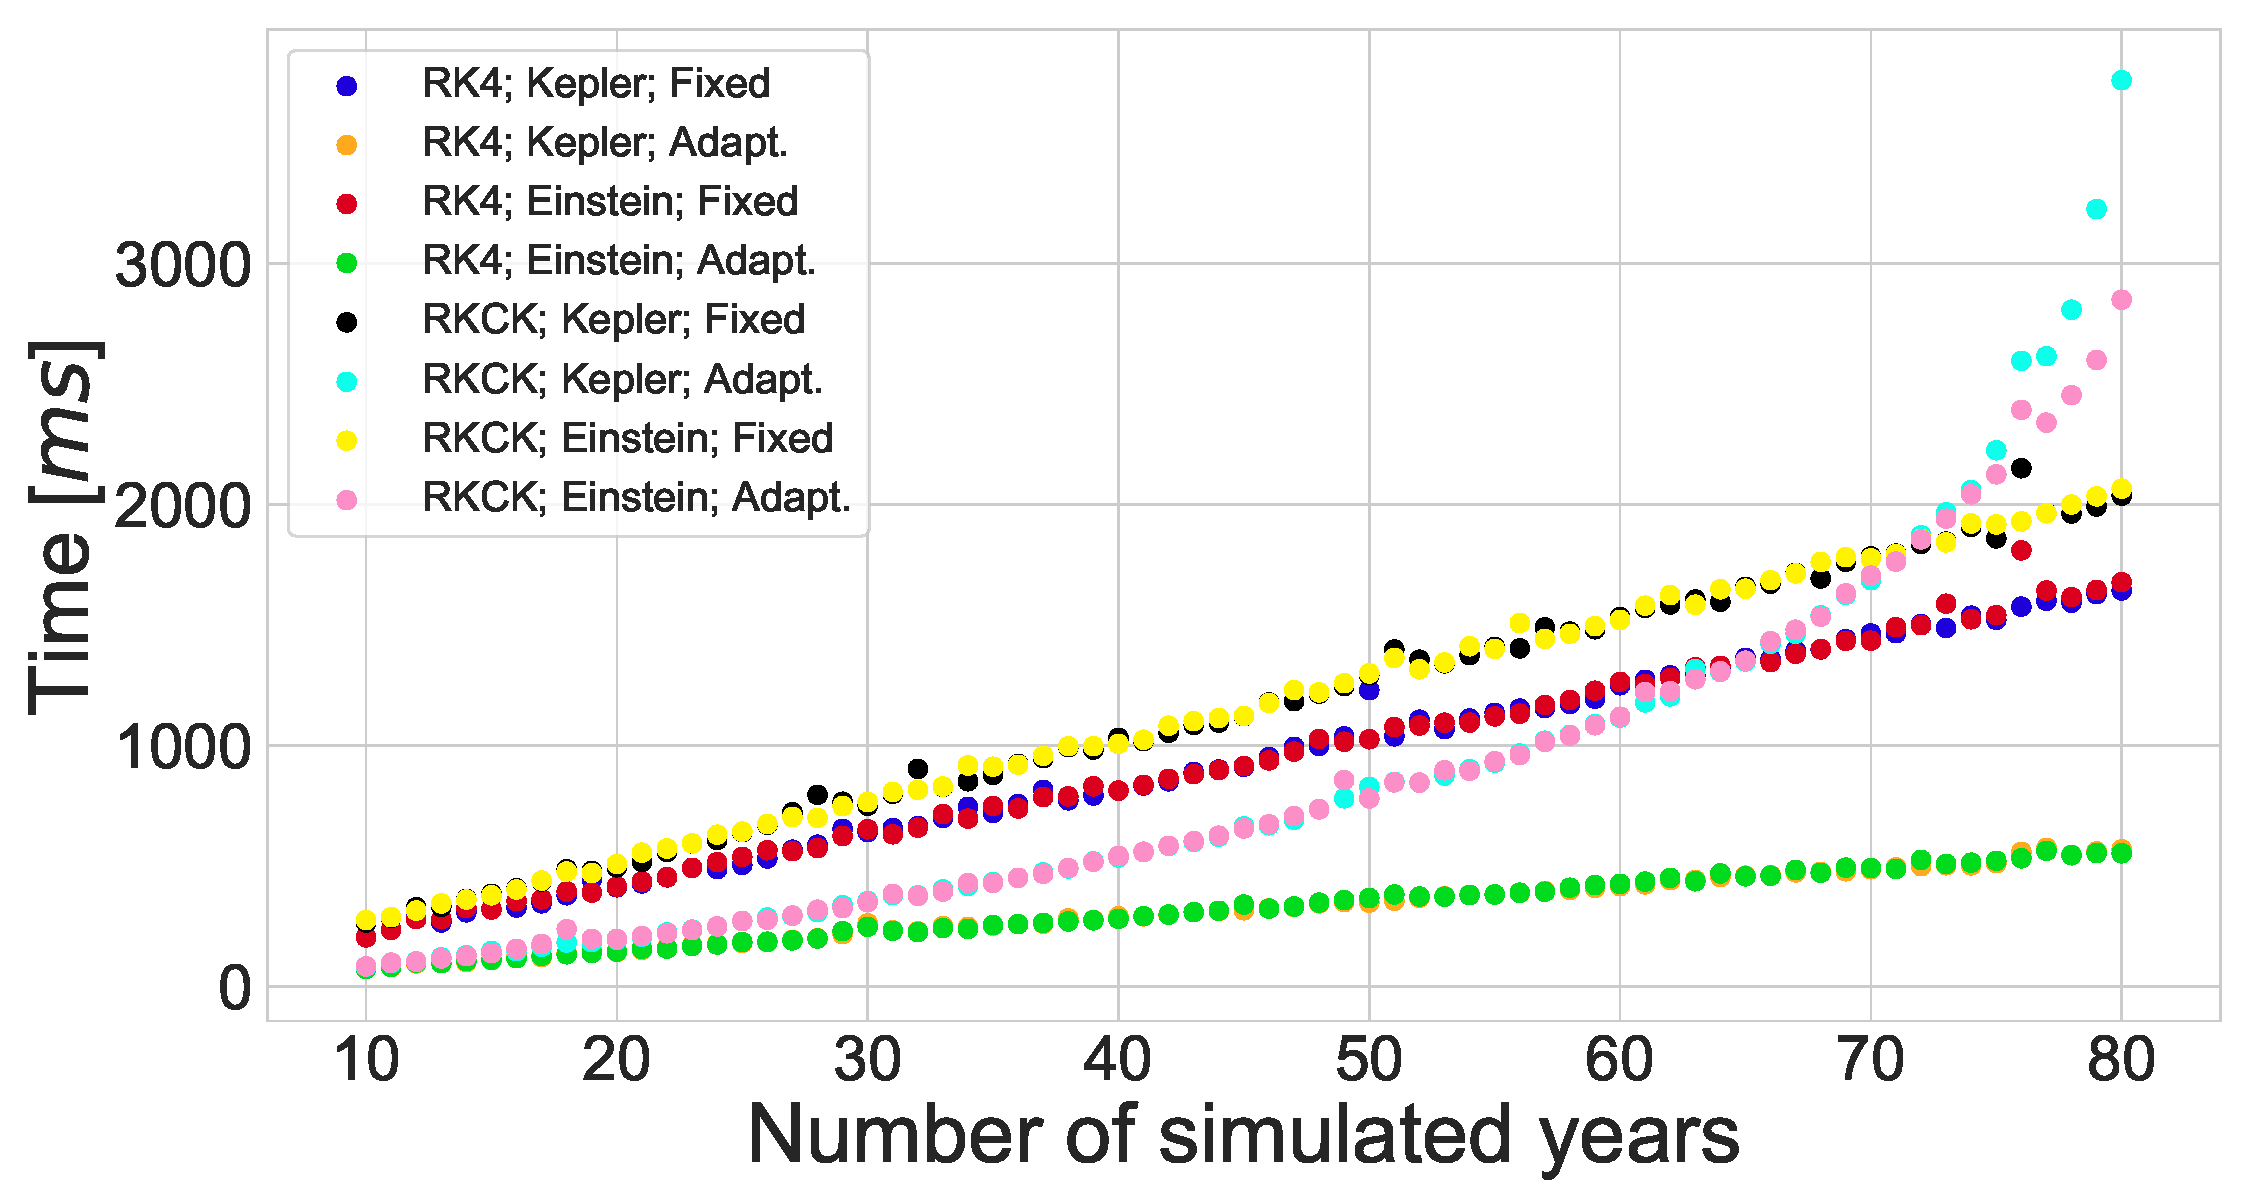
\includegraphics[width=0.5\textwidth]{images/single_body/runtime_all_1e-03.pdf}}
\captionof{figure}{Lépésköz nagysága $0.001 = 10^{-3}$ év}
\hfill \break \break
{\centering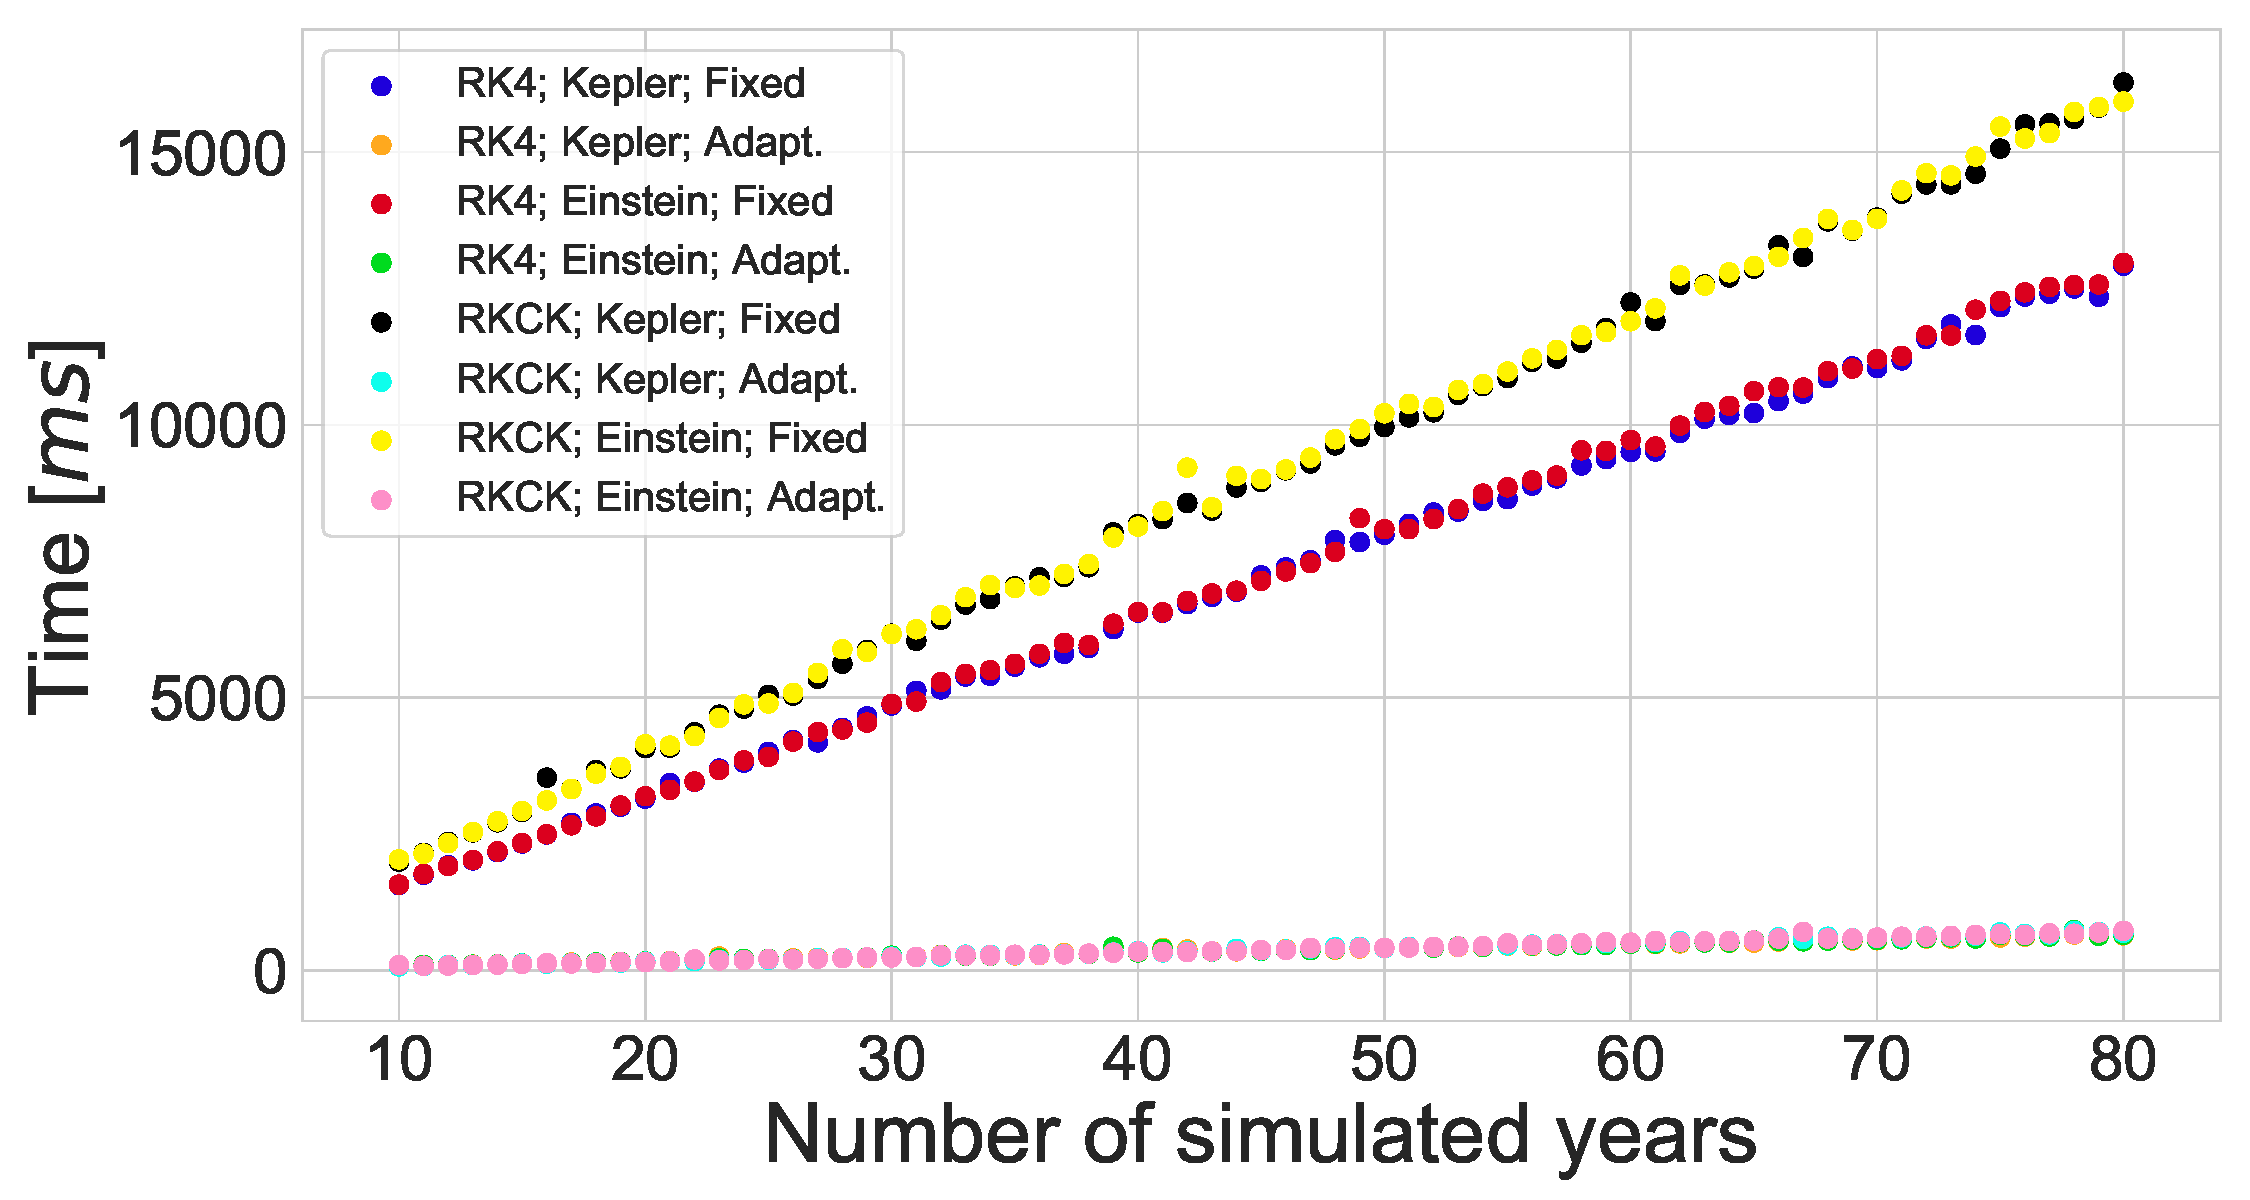
\includegraphics[width=0.5\textwidth]{images/single_body/runtime_all_1e-04.pdf}}
\captionof{figure}{Lépésköz nagysága $0.0001 = 10^{-4}$ év}
\hfill \break \break
Külön is ábrázoltam a nulla közelében elvesző adaptív integráló módszereket a jobb átláthatóság kedvéért:
\hfill \break \break
{\centering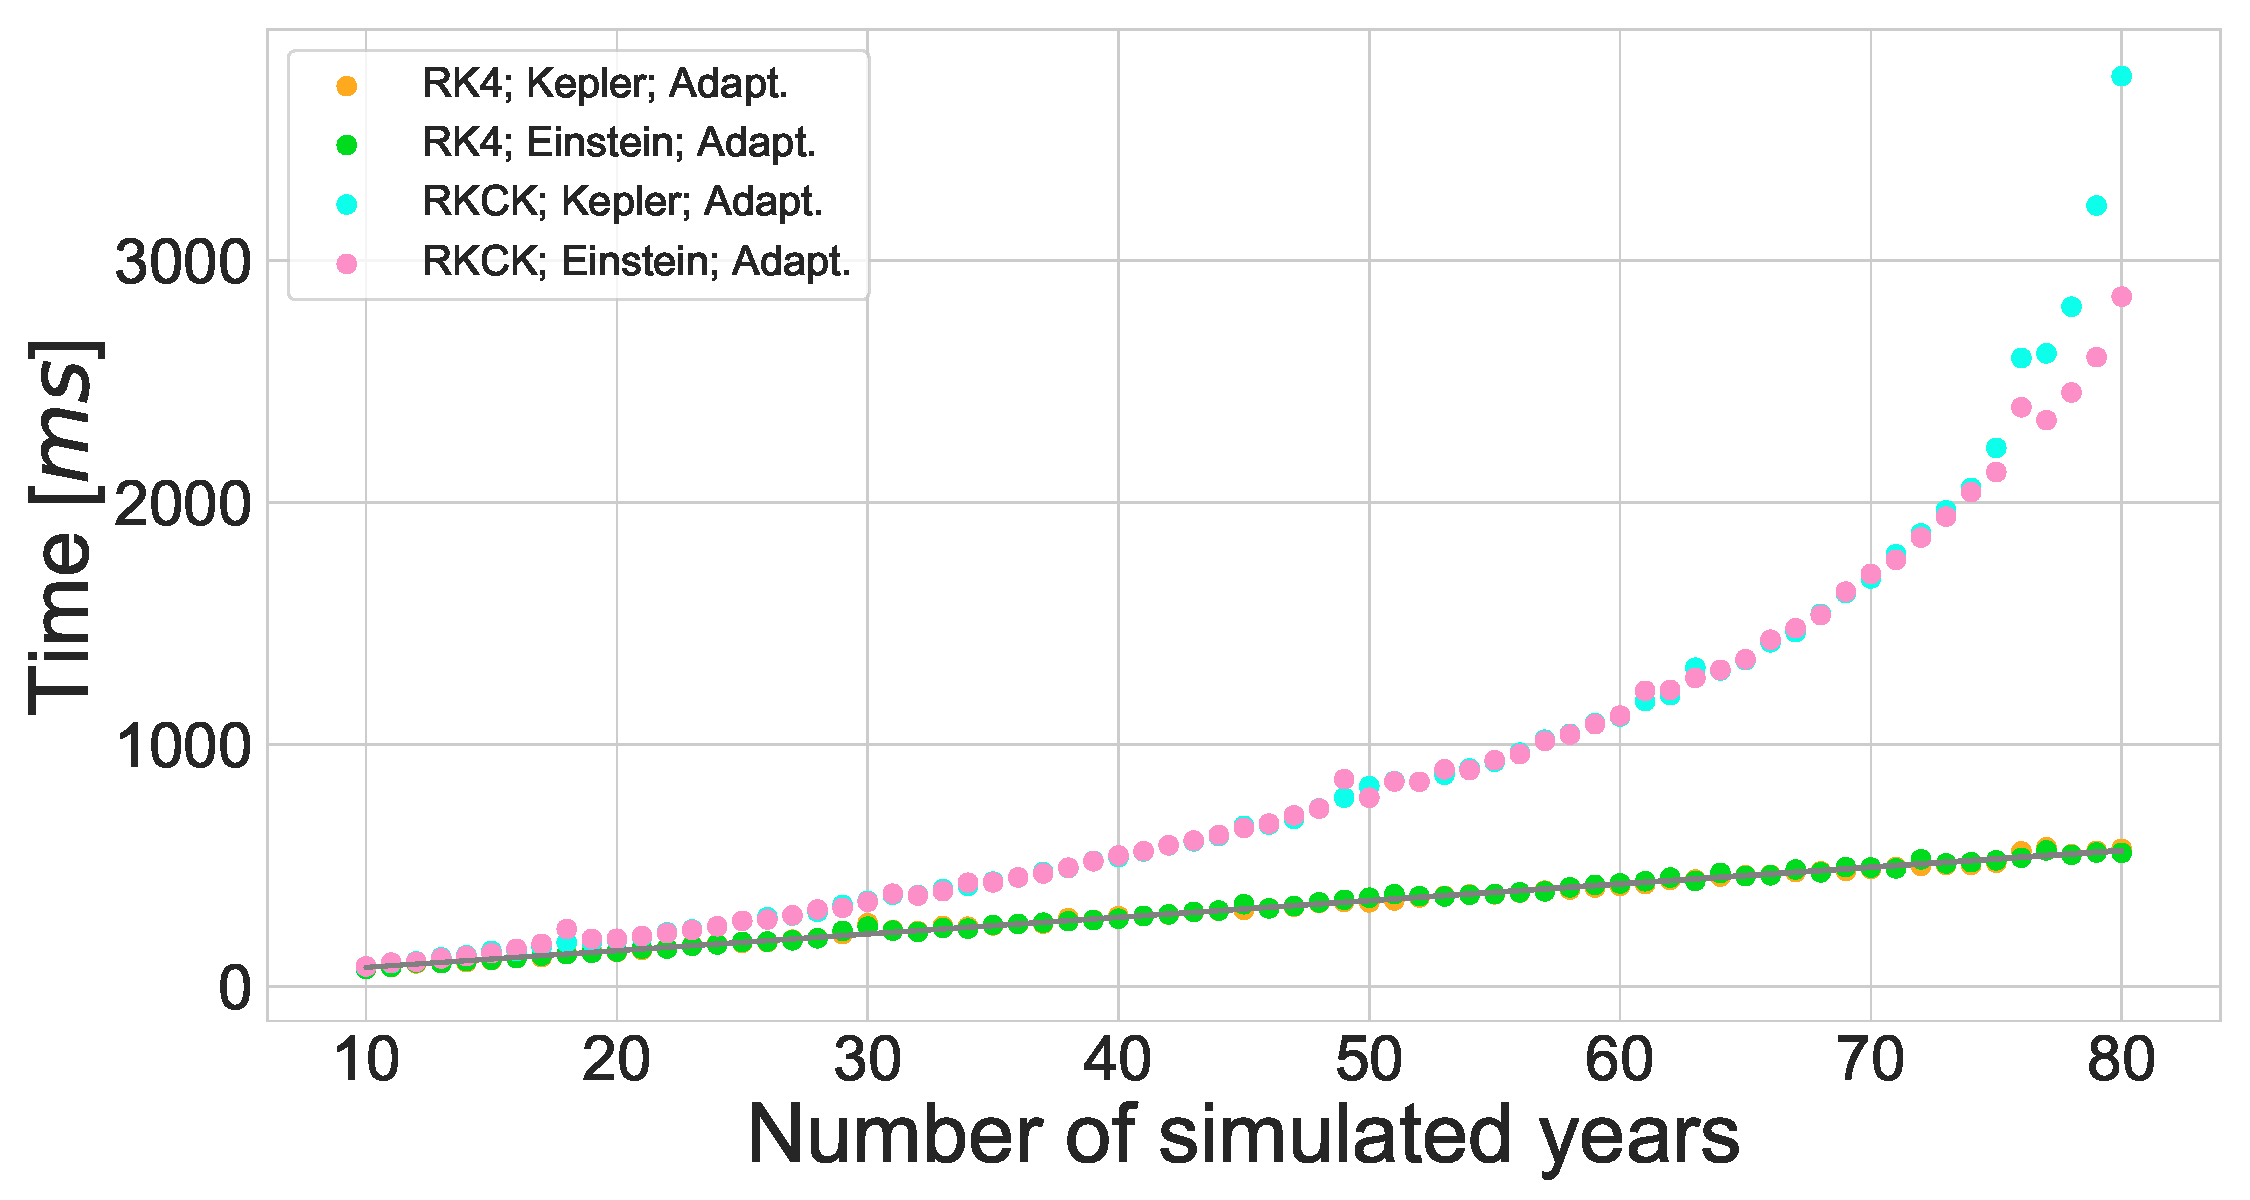
\includegraphics[width=0.5\textwidth]{images/single_body/runtime_adaptive_1e-03.pdf}}
\captionof{figure}{Adaptív integráló módszerek\\Lépésköz nagysága $0.001 = 10^{-3}$ év}
\hfill \break \break
{\centering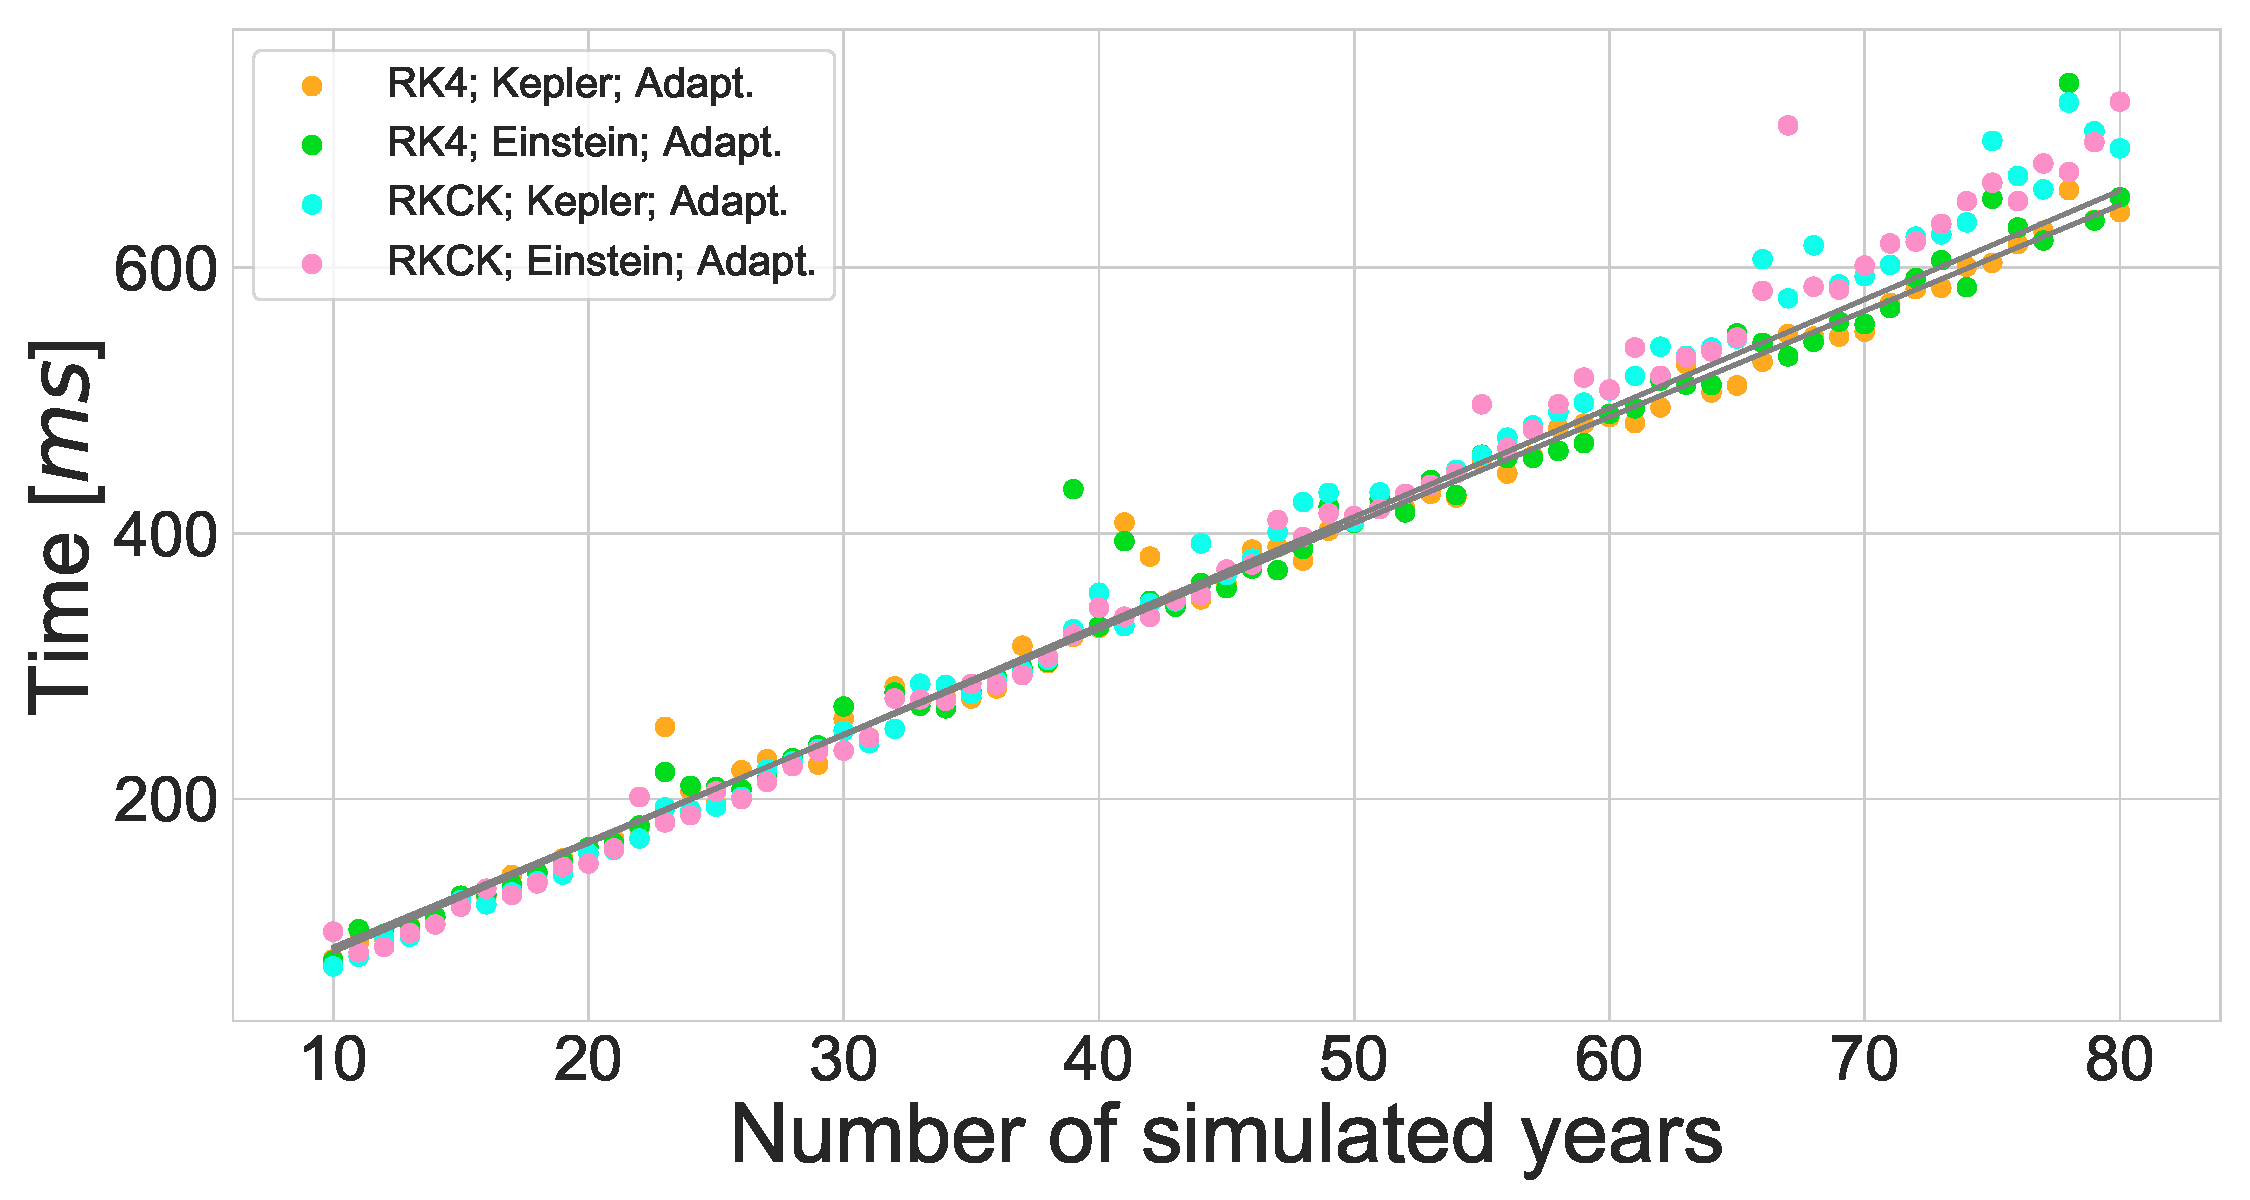
\includegraphics[width=0.5\textwidth]{images/single_body/runtime_adaptive_1e-04.pdf}}
\captionof{figure}{Adaptív integráló módszerek\\Lépésköz nagysága $0.0001 = 10^{-4}$ év}
\hfill \break \break
Ahogy vártuk, az adaptív lépéshosszal operáló módszerek gyorsabbak, hisz átlagosan mindig kevesebb lépést tettek meg a szimuláció során, adaptívan közelítve a Merkúr körpályáját. Szintén a vártaknak megfelelően a relativisztikus módszerek lassabban futnak le, mind a kepleri dinamikával operálók, ugyanis plusz két darab művelet szerepel benne a sebességkomponensek Lorentz-faktorokkal történő szorzása miatt. \\
Érdekes megfigyelni, hogy a Runge-Kutta-Cash-Karp algoritmusok $\text{dt} = 0.001 = 10^{-3}$ esetén valamiért futásidőben elszállnak, aminek az okát egyelőre nem tudtam megállapítani, ehhez további vizsgálatok szükségesek.

\section{Diszkusszió} \label{sec:5}
A szimuláció során megvizsgáltam annak numerikus stabilitását, megállapítottam, hogy kisebb ($10^{-3}-10^{-4}$) lépésköz esetén is előjönnek numerikus hibákból származó eltérések. Megállapítottam, hogy emiatt a Merkúr perihélium-precessziója a zajban elveszik, csak kisebb lépésközökkel, vagy a Lorentz-faktor súlyának manuális megválasztásával lehetne csak annak a tartományát elérni, amiket a hosszú futásidejük miatt már nem végeztem el. Ellenben a lépésköz $\text{dt}=10^{-5}$ megválasztásával már elértem valós adatokat használva a Merkúr precessziójának nagyságrendjét, és közelítő értékét.\\
Vizsgáltam az adaptív lépéshosszal operáló módszerek lépéshosszváltozását az időben előrehaladva. Megállapítottam azok karakterisztikáját és a választott pontosságok közti különbségeket, amiket a (\ref{sub:4.2}) részben ismertettem.\\
Végezetül a két- és háromtest-problémát oldottam meg, melyekről több animációt is készítettem, ugyanis a problémák és megoldásuk lényege legjobban azokon látszódhat. Ezeket meg is osztottam és elérhetővé tettem YouTube-on\cite{yt}.

\end{multicols}